\documentclass[
aspectratio=169 % comment for 4:3
]{beamer}


\usetheme[
hidetotal, % hide the total number of slides on the bottom right
hidenumbers, % hide current slide number
% hidename, % hide author name and title in footline
hidebullets, % use empty bullets in itemize
hidefootline, % hide the footline
%
% the previous options allow for a minimalistic style as recommended by Patrick
% Winston in his "how to speak" lecture at MIT
%
% sidebar, % show sidebar
hugetitle, % print main title in huge font
% thin, % use a thinner font
% bold, % use bold titles
% standardtitle, % use standard title slide (no picture)
]{mfrancois}

\setsecondarylogo{title/isia-logo} % Add a secondary logo to the title slide, optional
\settitleimage{title/raspberry} % Change the title slide image, optional (use images with a ratio identical to the one provided)

\author[F. Marelli]{François Marelli}
\affiliation[UMONS]{UMONS, ISIA Lab}
\title{Atelier Créactifs: Raspberry Pi}
\subtitle{Séance 1: Introduction}
\extras{
\includegraphics[height=25pt]{title/creactifs}}
\date{2 février 2026}

\graphicspath{{images}}

\begin{document}

\maketitle

\begin{frame}{\strut}
  \centering \alert{\huge Combien coûte un ordinateur?\strut}
\end{frame}

\begin{frame}{Un ordinateur à 10€?}
  \centering
  \vspace{1em}
  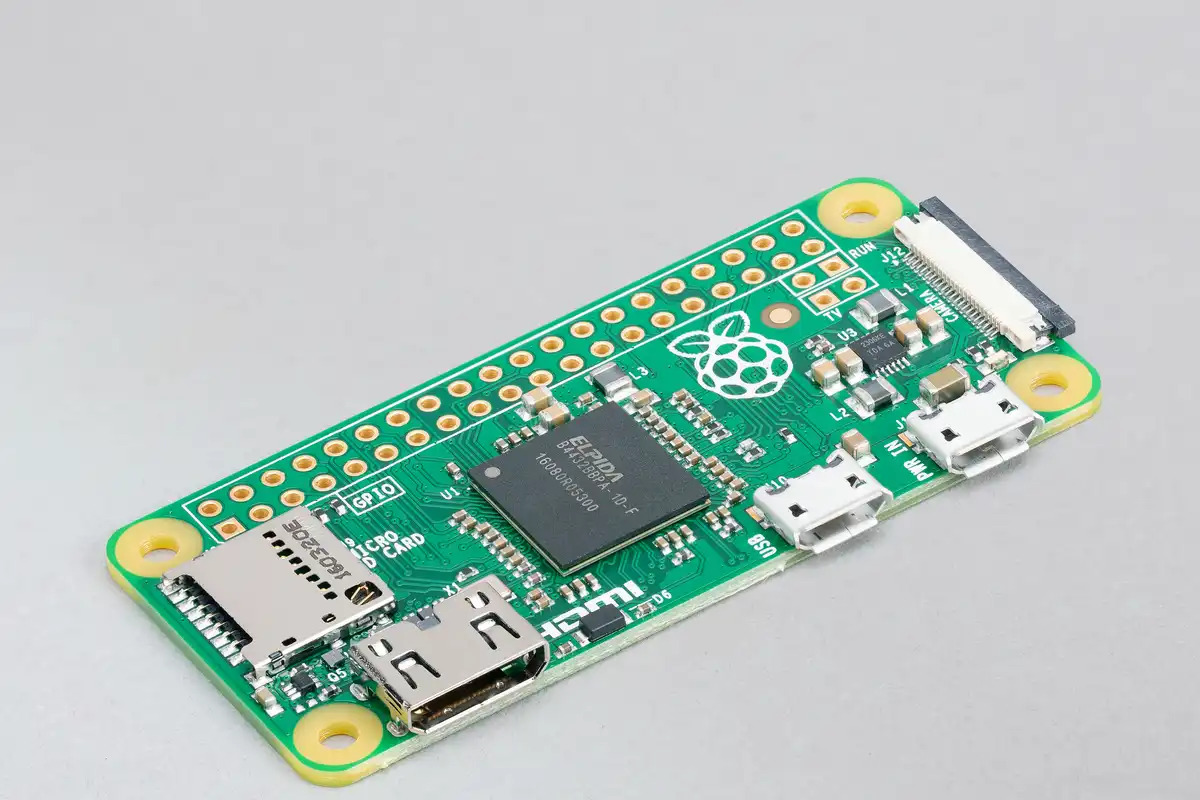
\includegraphics[width=.7\textwidth]{pizero}

  \tiny{Source: raspberrypi.com}
\end{frame}

\begin{frame}{La famille Raspberry Pi}
  \begin{columns}
    \begin{column}{0.55\textwidth}
      \centering
      \vspace{1em}
      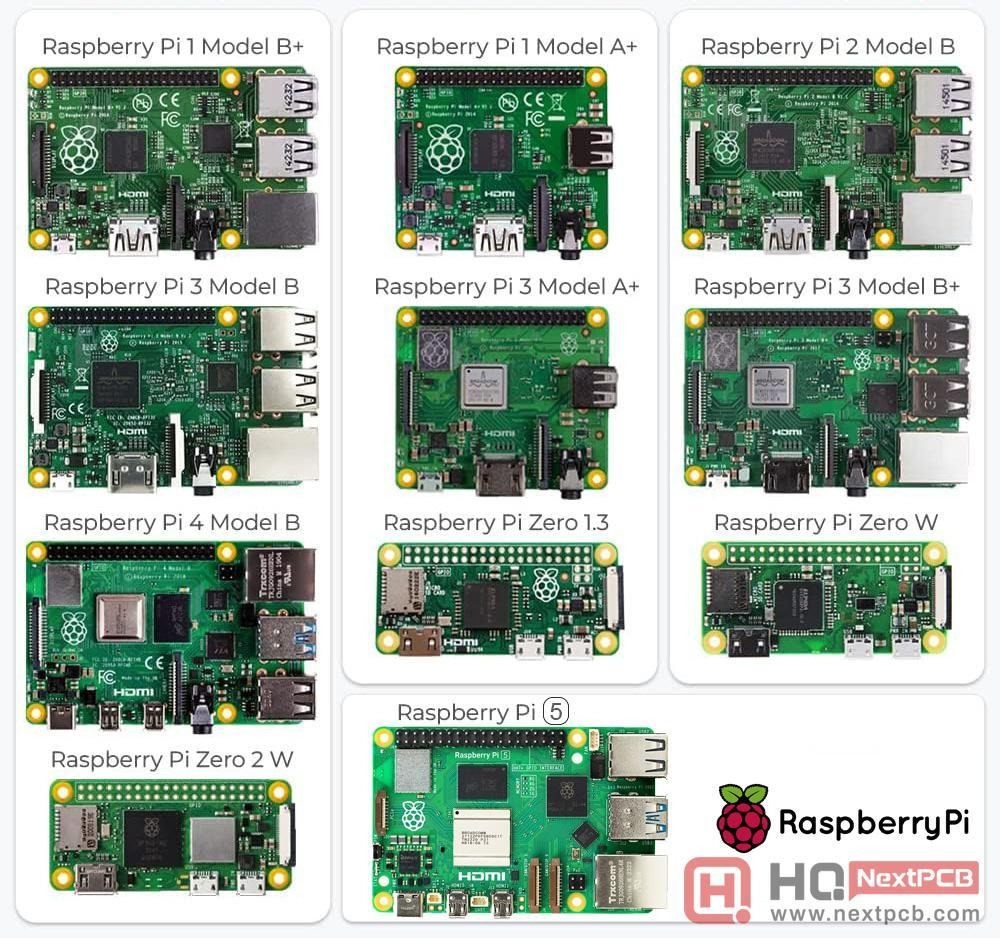
\includegraphics[width=.9\textwidth]{pi-family}

      \tiny{Source:nextpcb.com}
    \end{column}
    \begin{column}{0.5\textwidth}
      Différents modèles, plus ou moins:
      \begin{itemize}
        \item récents (2012-2023)
        \item chers (10-200€)
        \item puissants (CPU, RAM)
      \end{itemize}

      \bigskip \alert{Pour ce cours: Raspberry Pi 3B (2016, 40€)}
    \end{column}
  \end{columns}

\end{frame}

\begin{frame}{Visite guidée du Raspberry Pi 3B}{Attention au risque
    électrostatique} \vspace{1em} \centering \alert{\huge On touche du métal!
  }

  Et on touche du bois que ça suffise
\end{frame}

\begin{frame}{Visite guidée du Raspberry Pi 3B}{4x USB 2} \centering
  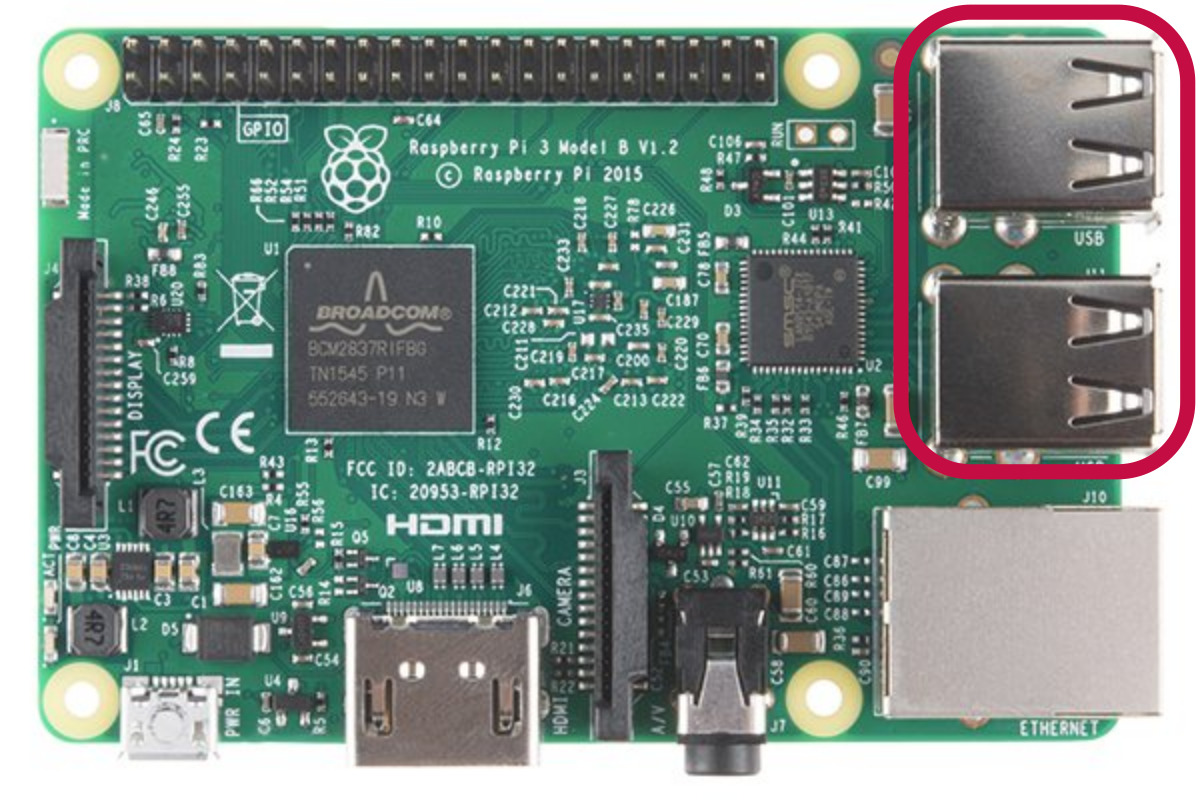
\includegraphics[width=.7\textwidth]{components_usb}
\end{frame}
\begin{frame}{Visite guidée du Raspberry Pi 3B}{Ethernet 100Mbps} \centering
  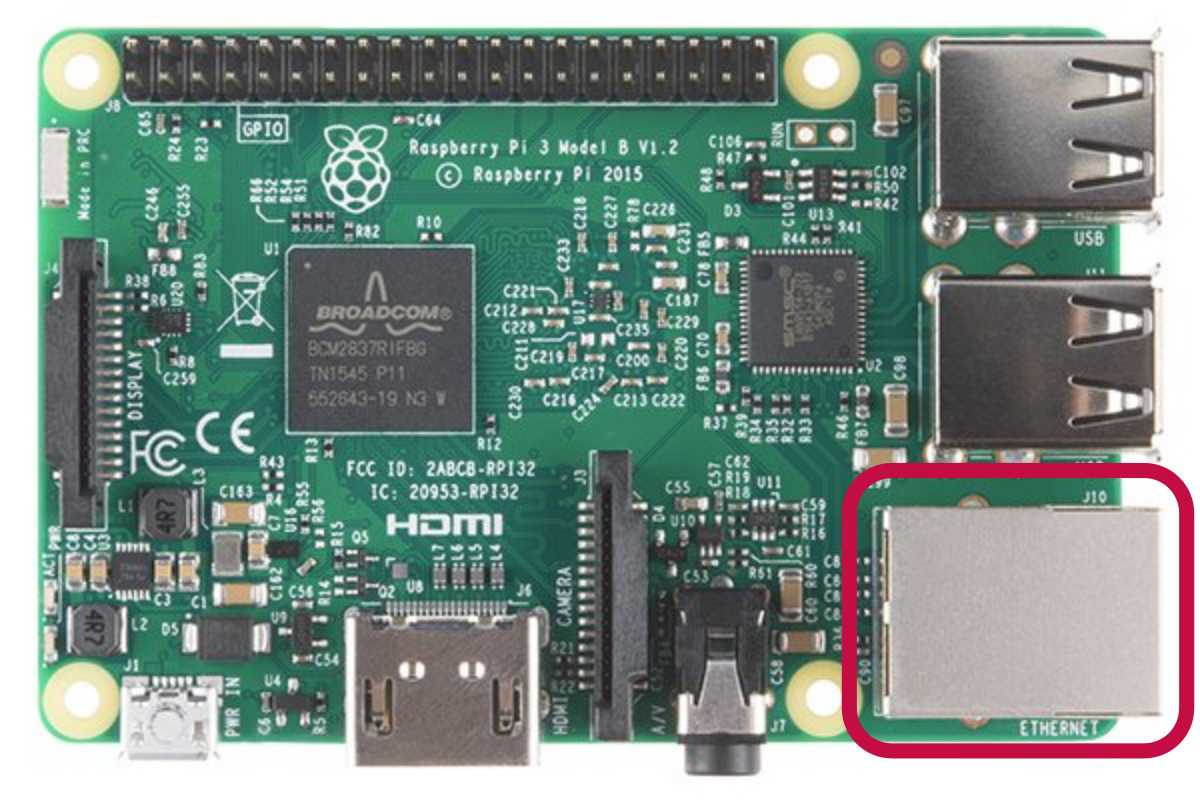
\includegraphics[width=.7\textwidth]{components_ethernet}
\end{frame}
\begin{frame}{Visite guidée du Raspberry Pi 3B}{Jack audio} \centering
  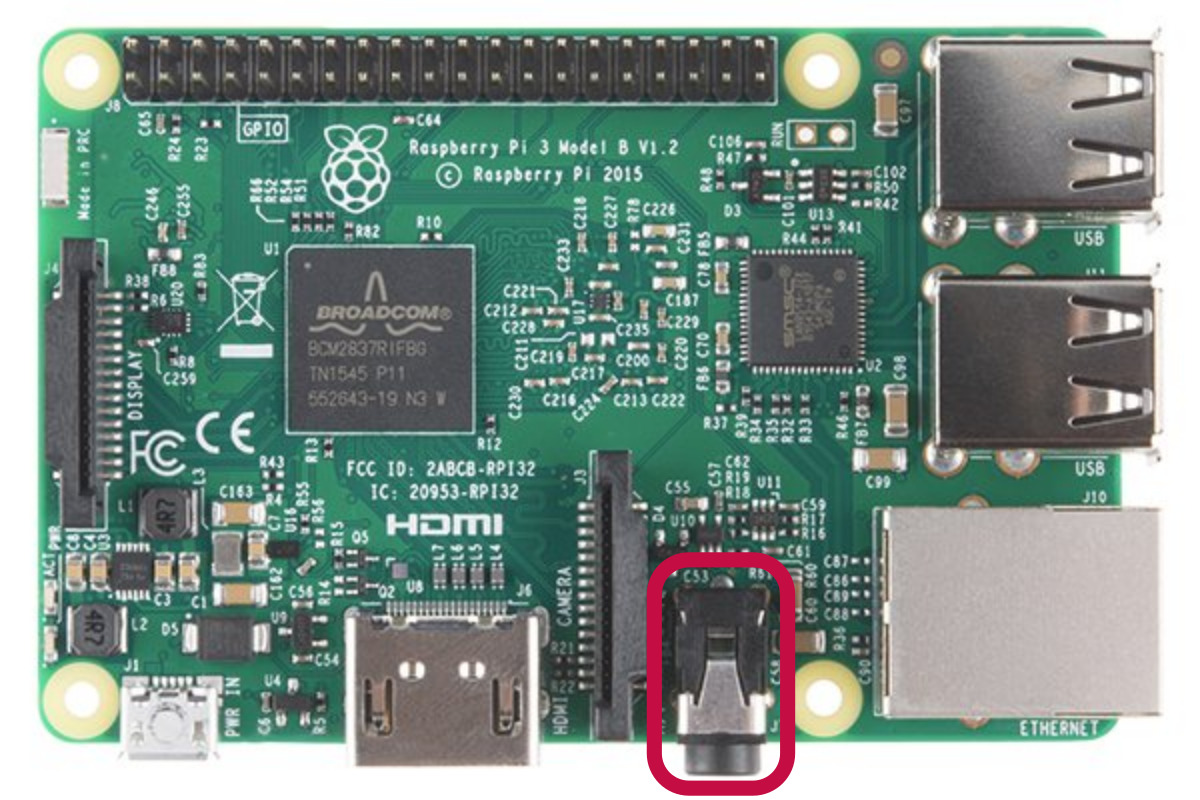
\includegraphics[width=.7\textwidth]{components_jack}
\end{frame}
\begin{frame}{Visite guidée du Raspberry Pi 3B}{HDMI} \centering
  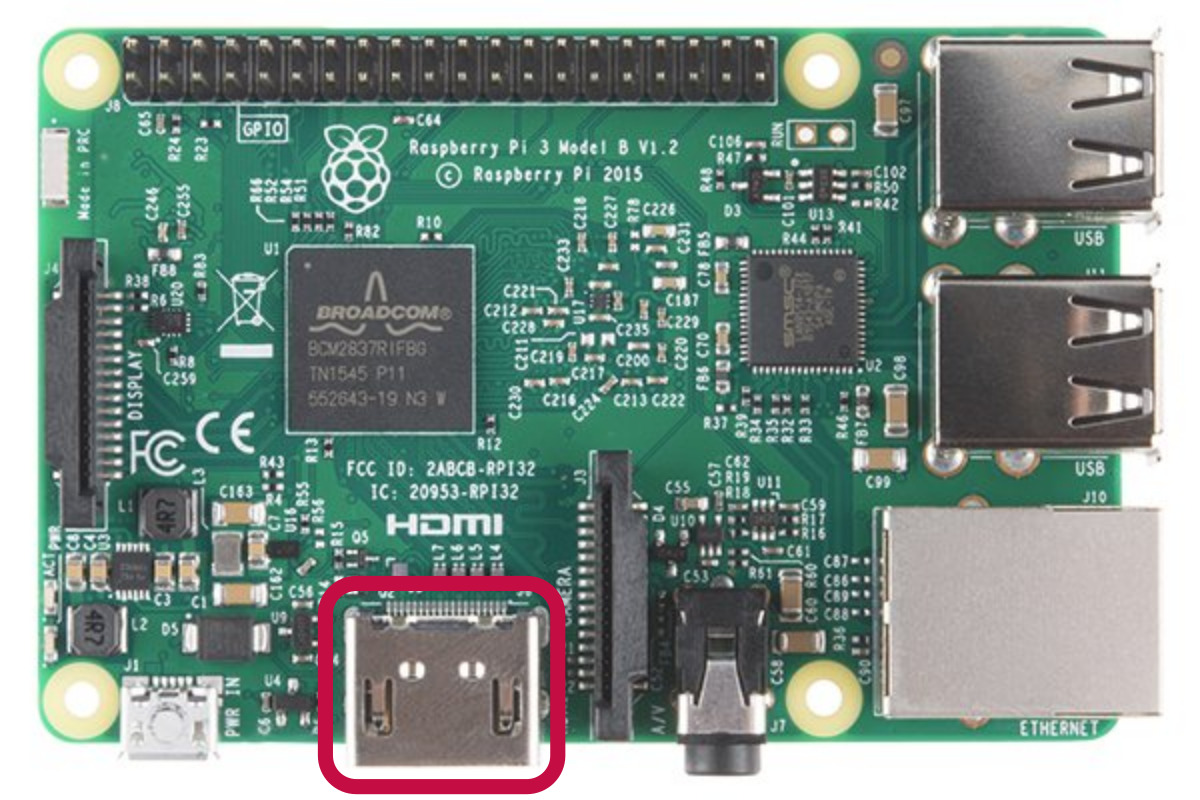
\includegraphics[width=.7\textwidth]{components_hdmi}
\end{frame}
\begin{frame}{Visite guidée du Raspberry Pi 3B}{Micro USB (alimentation)}
  \centering 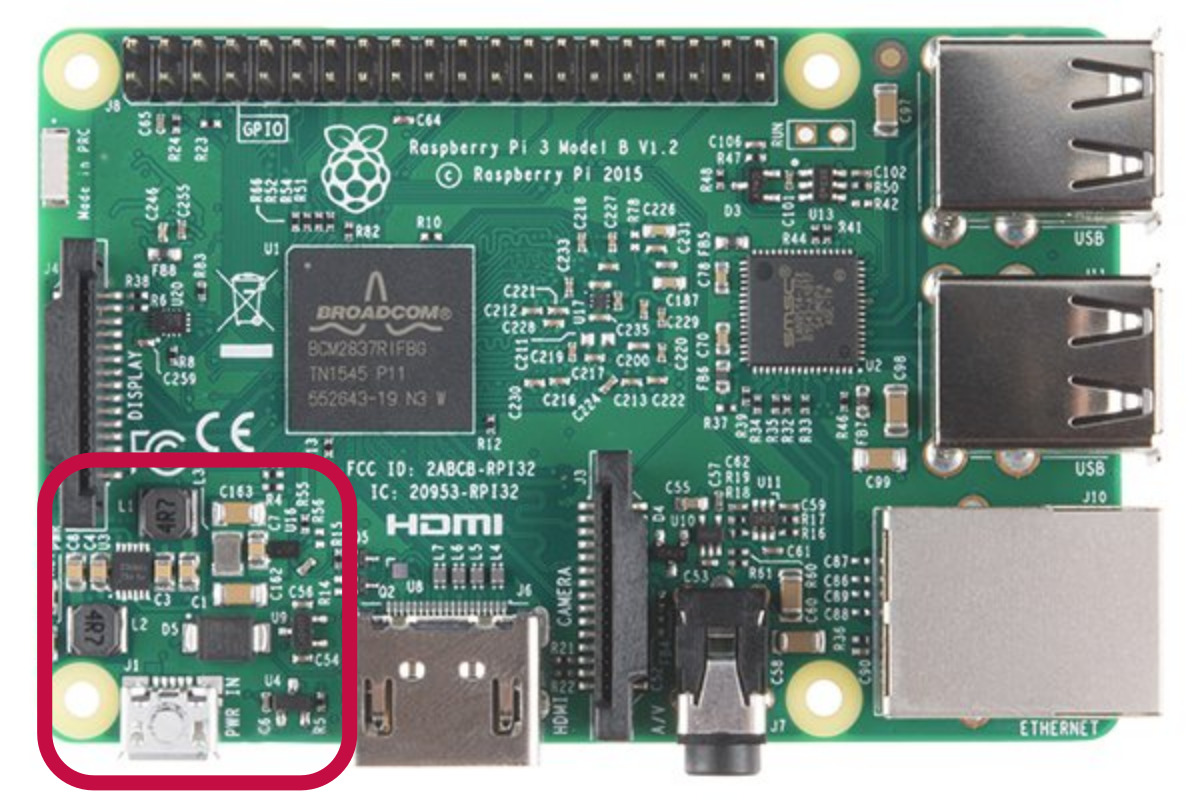
\includegraphics[width=.7\textwidth]{components_power}
\end{frame}
\begin{frame}{Visite guidée du Raspberry Pi 3B}{Ecran DSI / caméa CSI}
  \centering 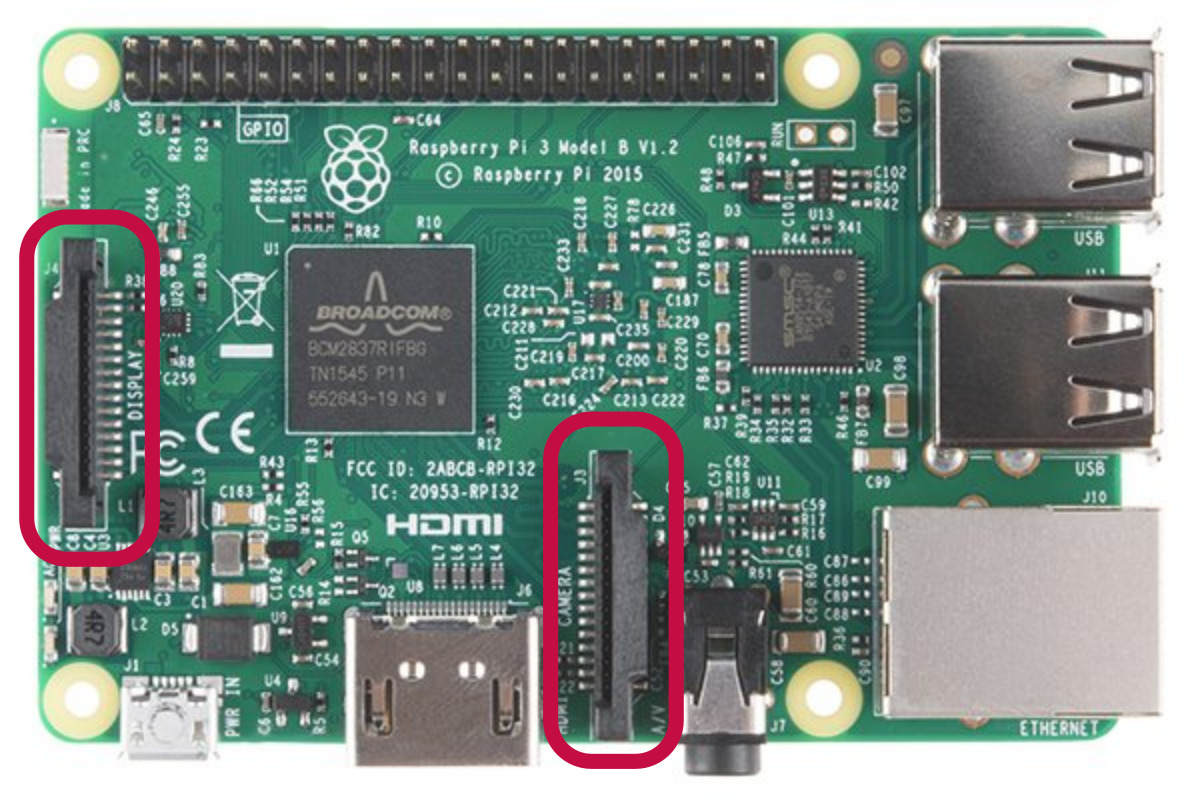
\includegraphics[width=.7\textwidth]{components_camera}
\end{frame}
\begin{frame}{Visite guidée du Raspberry Pi 3B}{GPIO} \centering
  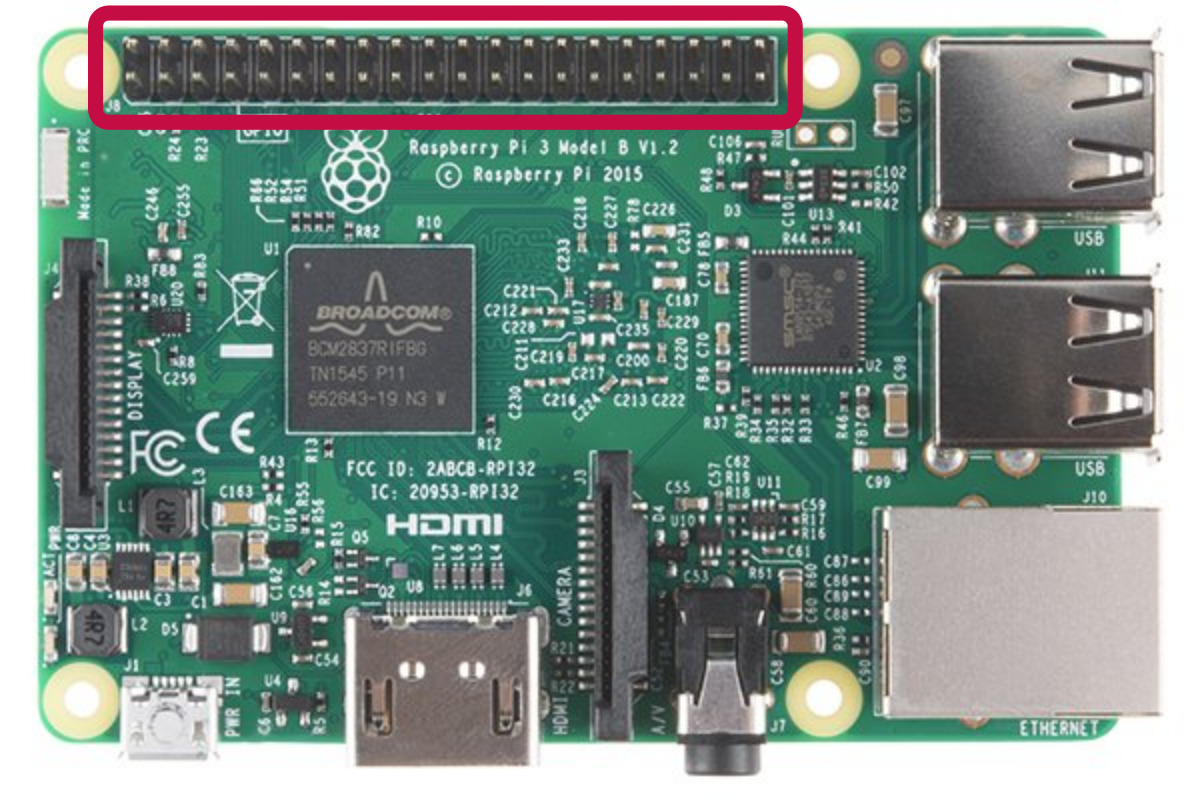
\includegraphics[width=.7\textwidth]{components_gpio}
\end{frame}
\begin{frame}{Visite guidée du Raspberry Pi 3B}{CPU + GPU} \centering
  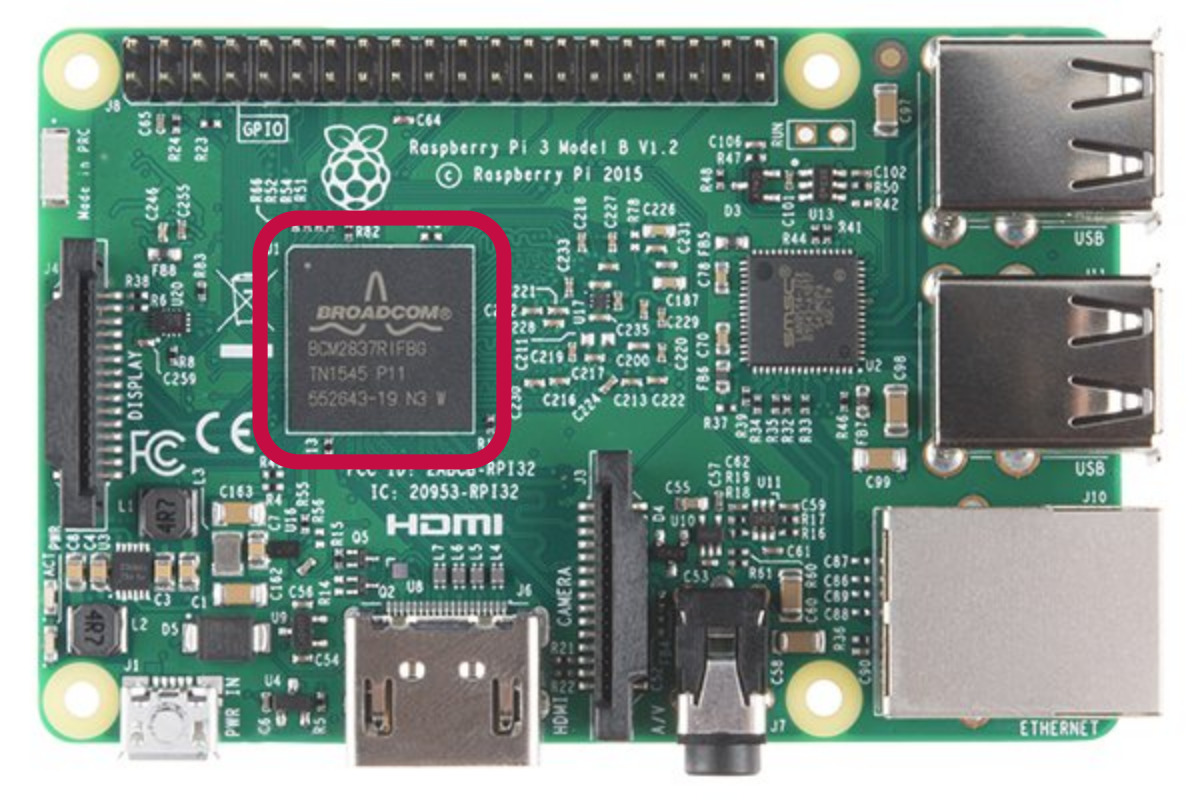
\includegraphics[width=.7\textwidth]{components_cpu}
\end{frame}
\begin{frame}{Visite guidée du Raspberry Pi 3B}{Contrôleur USB/Ethernet}
  \centering 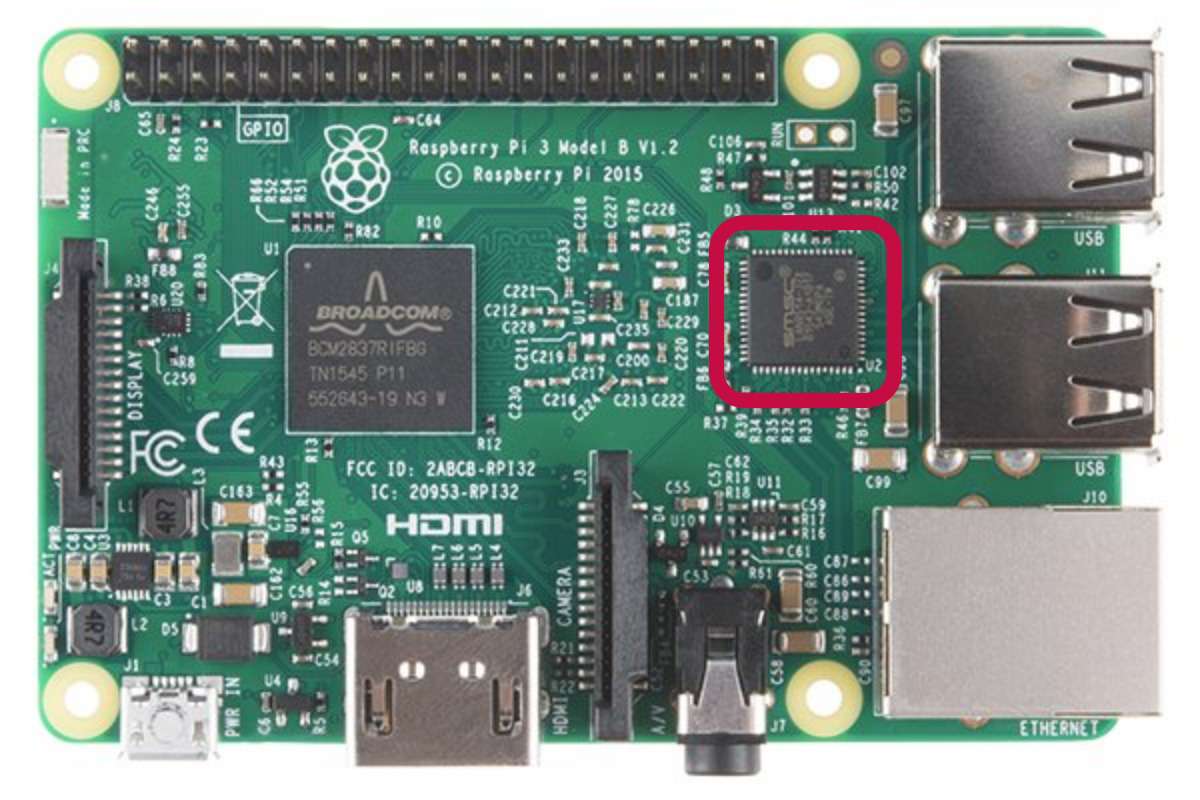
\includegraphics[width=.7\textwidth]{components_hub}
\end{frame}
\begin{frame}{Visite guidée du Raspberry Pi 3B}{Antenne Wi-Fi/Bluetooth}
  \centering 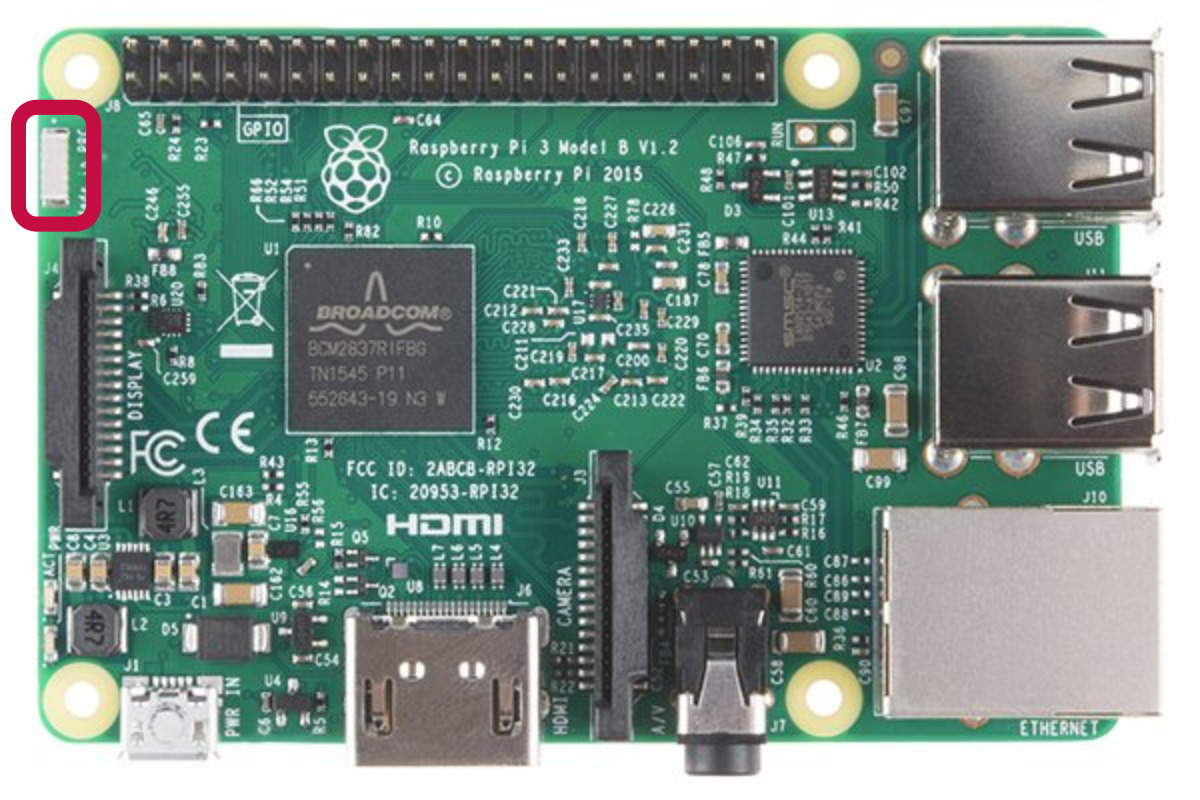
\includegraphics[width=.7\textwidth]{components_antenna}
\end{frame}
\begin{frame}{Visite guidée du Raspberry Pi 3B}{Points de montage} \centering
  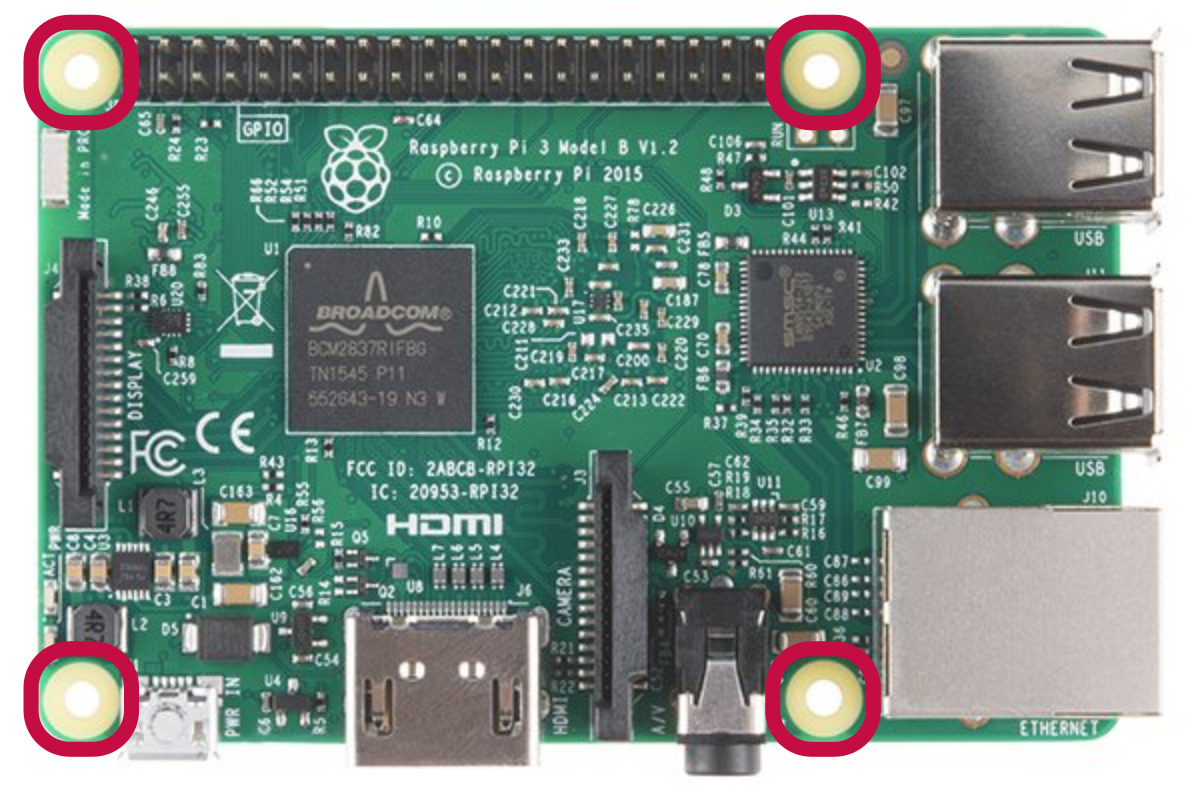
\includegraphics[width=.7\textwidth]{components_mounting}
\end{frame}

\begin{frame}{Visite guidée du Raspberry Pi 3B}{Lecteur de carte micro-SD}
  \centering 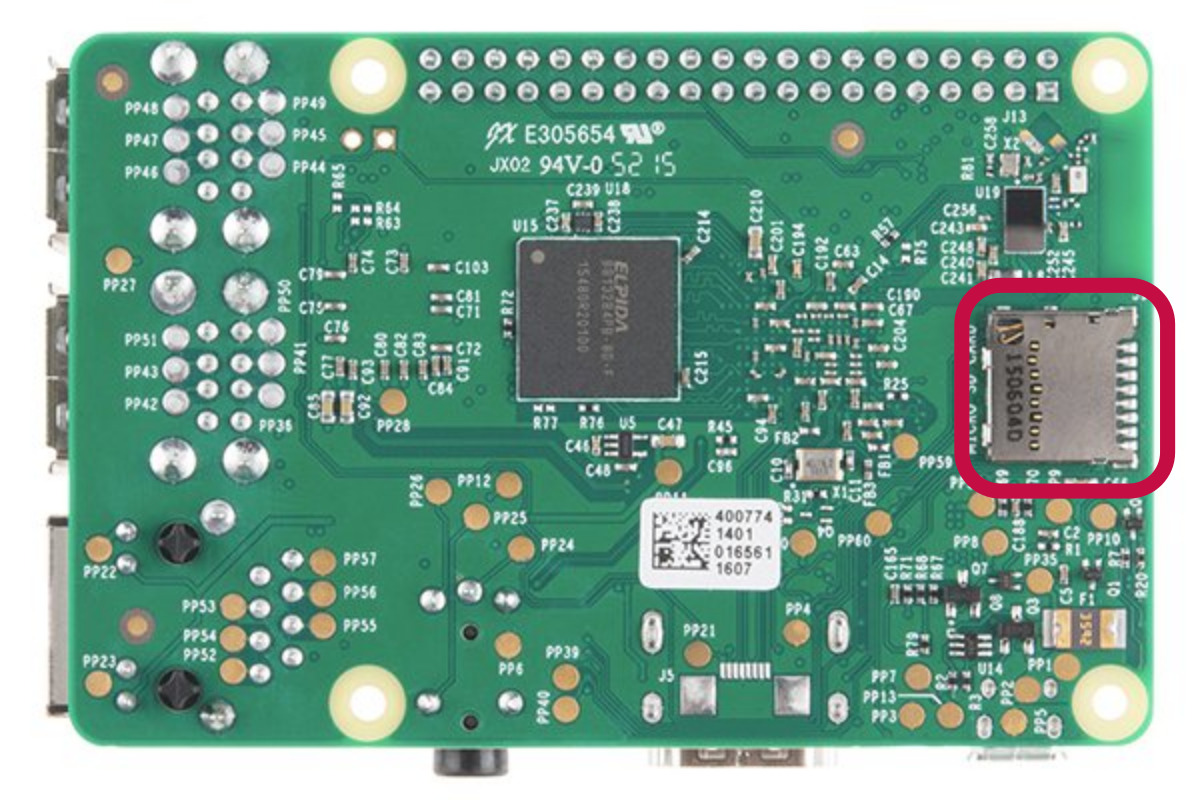
\includegraphics[width=.7\textwidth]{components_sd}
\end{frame}
\begin{frame}{Visite guidée du Raspberry Pi 3B}{Mémoire RAM} \centering
  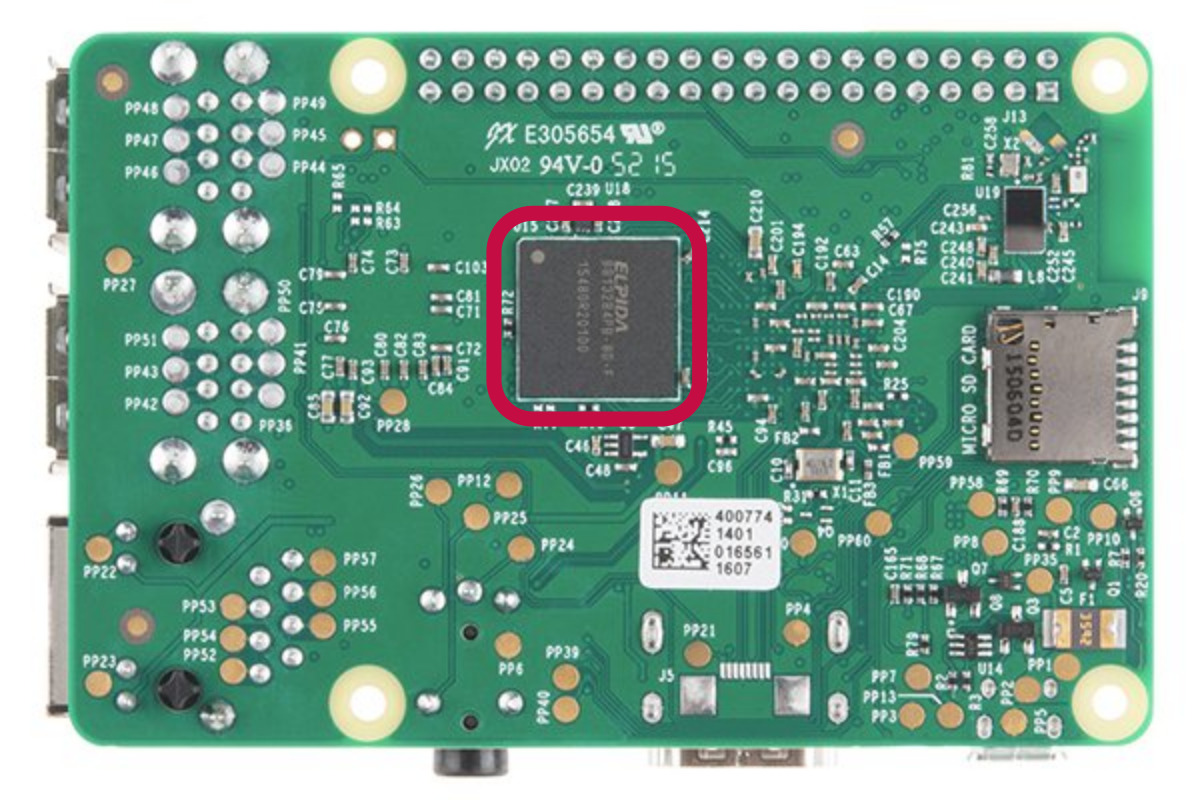
\includegraphics[width=.7\textwidth]{components_ram}
\end{frame}
\begin{frame}{Visite guidée du Raspberry Pi 3B}{Contrôleur Wi-Fi/Bluetooth}
  \centering 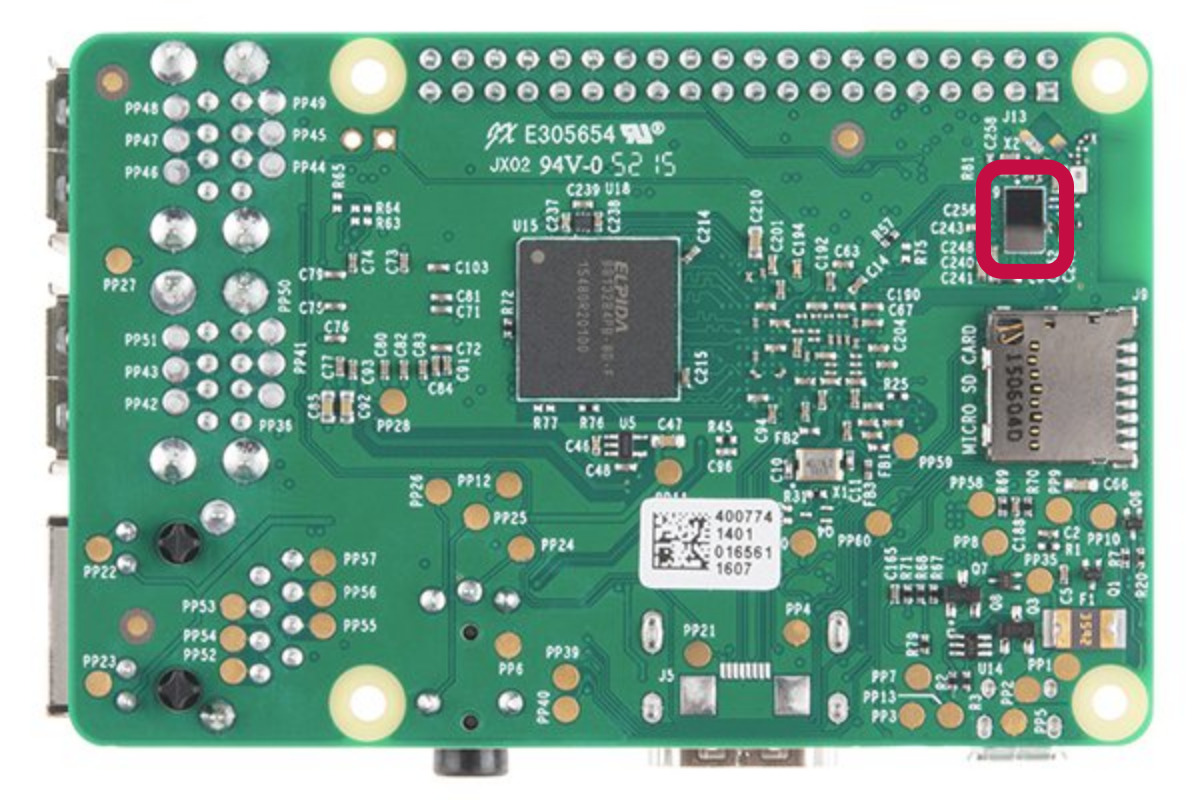
\includegraphics[width=.7\textwidth]{components_wifi}
\end{frame}

\begin{frame}{SBC: ordinateur à carte unique}{Une carte pour les gouverner
    toutes\ldots}
  \begin{columns}
    \begin{column}{.5\textwidth}
      \begin{block}{Avantages}
        \begin{itemize}
          \item Prix inférieur
          \item Compacité
          \item Faible consommation (1-5W, 10x moins)
          \item Flexibilité (GPIO)

        \end{itemize}

      \end{block}
    \end{column}
    \begin{column}{.5\textwidth}
      \begin{alertblock}{Inconvénients}
        \begin{itemize}
          \item Puissance de calcul
                limitée
          \item Mémoire RAM limitée
          \item Besoin d'accessoires
          \item Stockage SD
                (lent, fragile)
        \end{itemize}
      \end{alertblock}
    \end{column}
  \end{columns}

  \bigskip \bigskip \bigskip \centering \alert{\(\rightarrow\) Parfait pour des
    projets DIY, embarqués ou qui tournent en continu!
  }
\end{frame}

\begin{frame}{Plan de l'atelier}
  8 séances, 1 objectif: \alert{créer son propre petit serveur de maison!}

  \bigskip
  \begin{itemize}
    \item[02/02] Introduction à Raspberry Pi
    \item[09/02] Exploration du terminal Linux
    \item[02/03] Programmation Python, GPIO et capteurs
    \item[09/03] Utilisation de la caméra et de l'écran tactile
    \item[16/03] Découverte de la domotique
    \item[23/03] Création d'un serveur multimédia
    \item[30/03] Bases en réseau et VPN
    \item[06/04] Bonus et projets libres
  \end{itemize}
\end{frame}

\begin{frame}{Philosophie de l'atelier}{Et de l'enseignant\ldots}

  Qui suis-je?
  \begin{itemize}
    \item François (on peut se tutoyer?)
    \item Chercheur dans les technologies de la médecine
    \item Amateur de DIY électronique et informatique
  \end{itemize}

  \bigskip
  "Règles" du cours:
  \begin{itemize}
    \item Respect mutuel et du matériel
    \item
          Interrompez-moi, posez des questions
    \item Amusez-vous, proposez vos idées
  \end{itemize}

  \bigskip
  Qui êtes-vous?

\end{frame}

\begin{frame}{On dirait une Arduino?
  }{De loin\ldots}
  \begin{columns}
    \begin{column}{.6\textwidth}
      \centering
      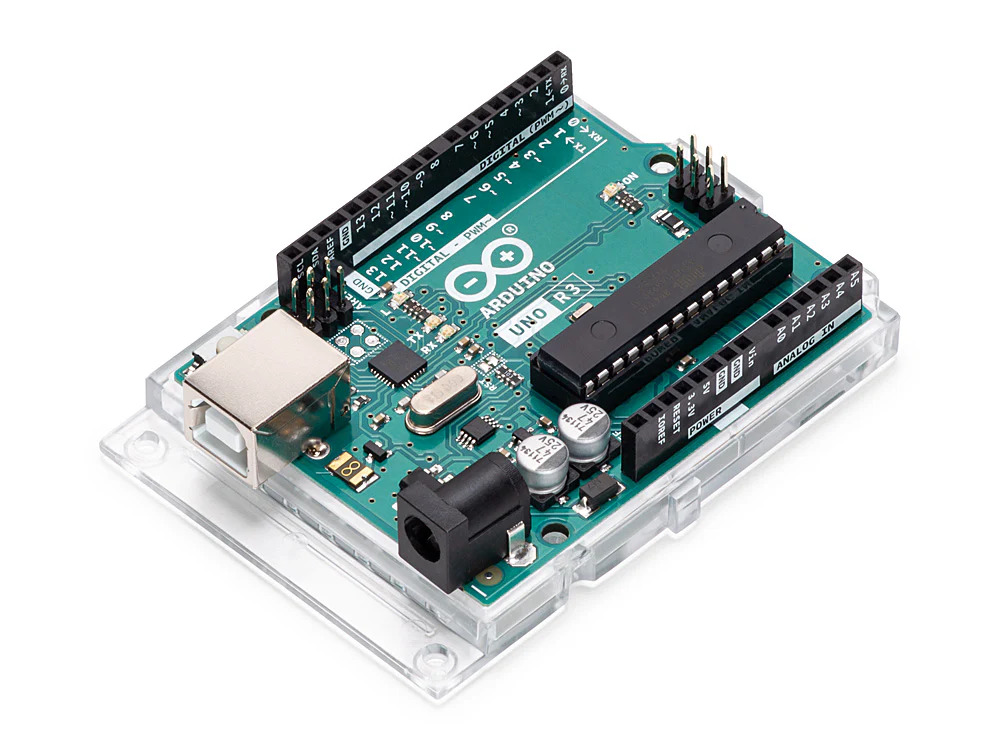
\includegraphics[width=.9\textwidth]{arduino}

      \tiny{Source: arduino.cc}
    \end{column}
    \begin{column}{.4\textwidth}
      SBC \(\neq\) Microcontrôleur:
      \begin{itemize}
        \item plus puissant
        \item plus
              complexe
        \item plus flexible
        \item pas temps réel
        \item \alert{système
                d'exploitation}
      \end{itemize}
    \end{column}
  \end{columns}
\end{frame}

\begin{frame}{Le système d'exploitation}
  \begin{columns}
    \begin{column}{.5\textwidth} \centering 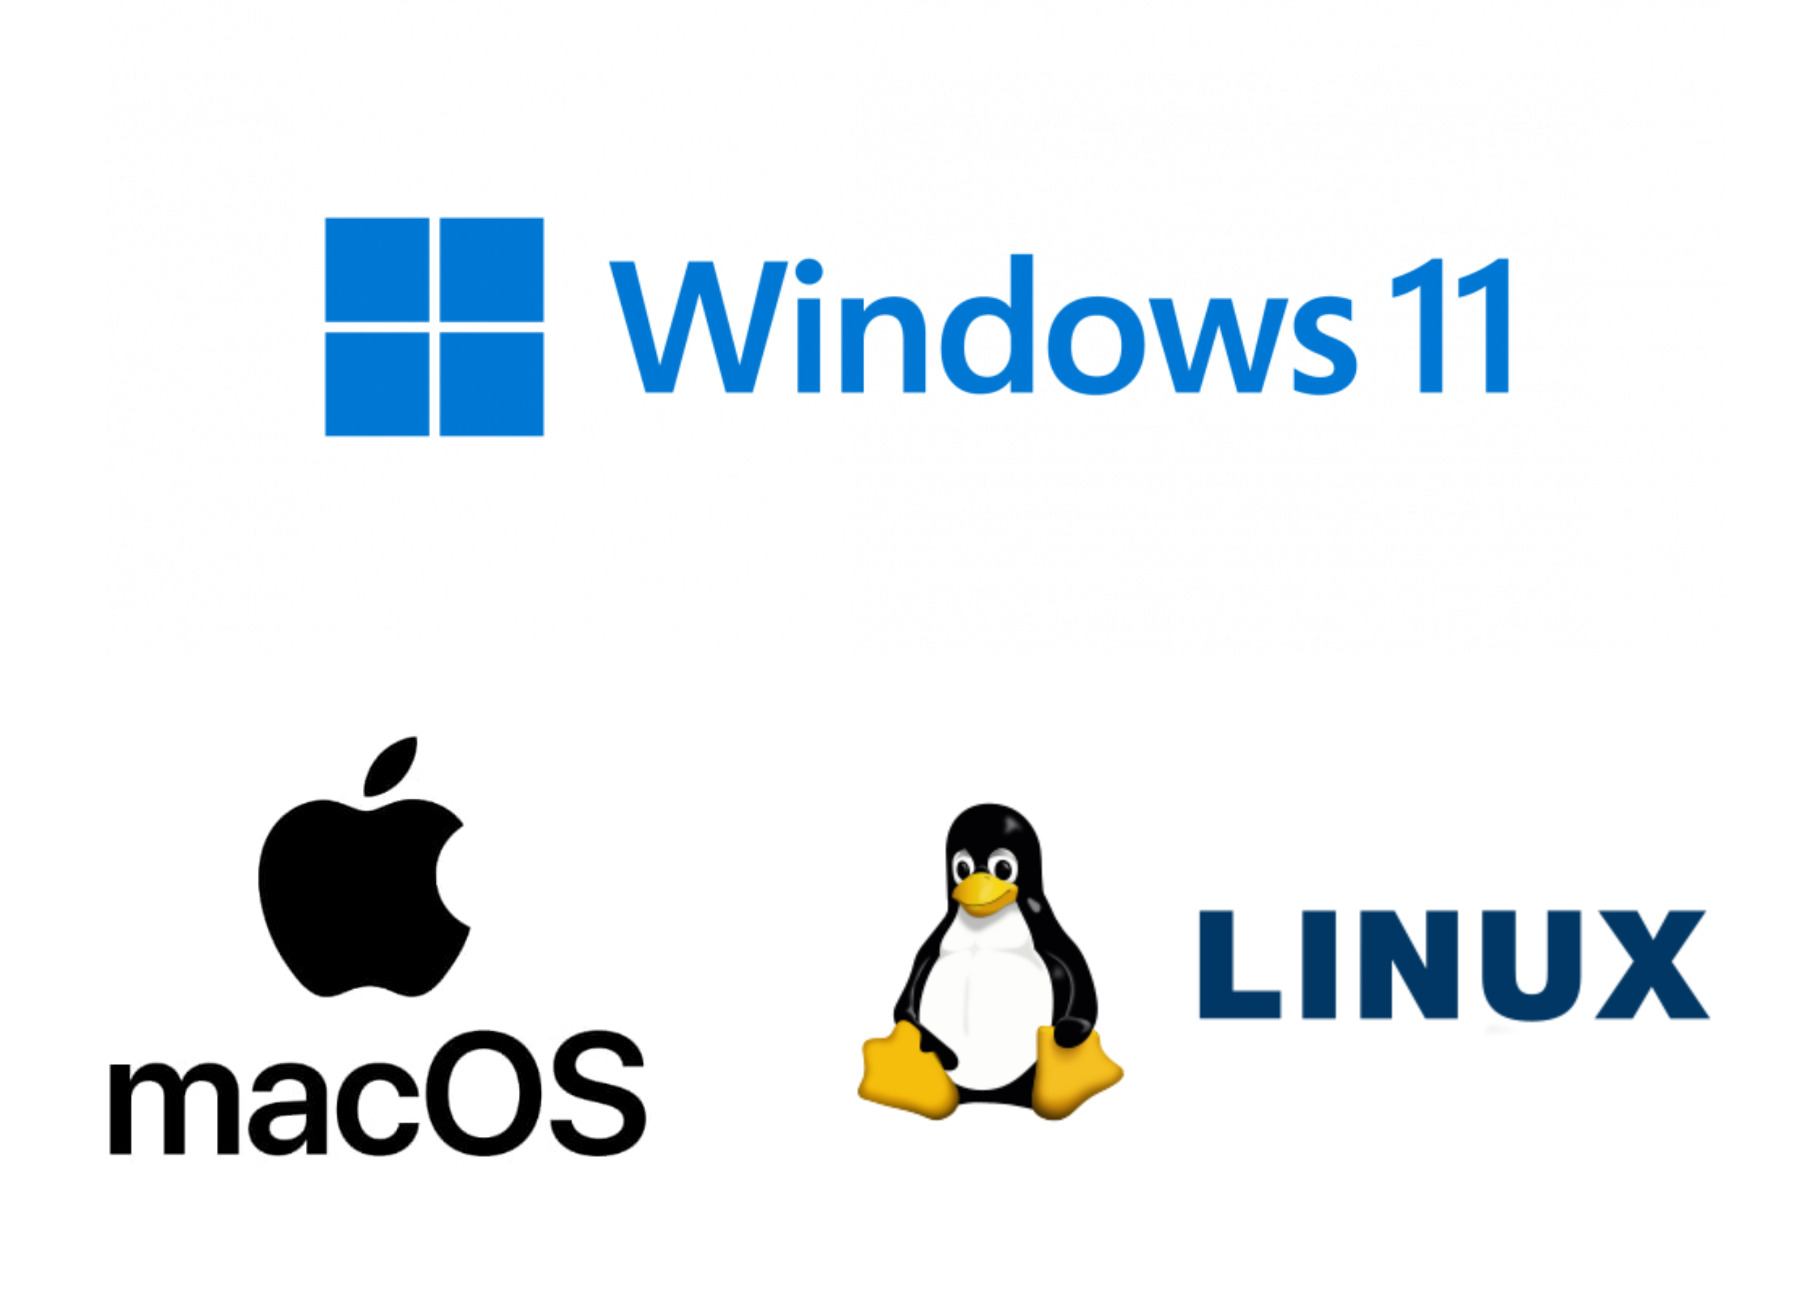
\includegraphics[width=.9\textwidth]{os}
    \end{column}
    \begin{column}{.5\textwidth} Qu'est-ce qu'un système
      d'exploitation?
      \begin{itemize}
        \item Interface utilisateur - matériel
        \item Gestionnaire de ressources
        \item Environnement d'exécution
      \end{itemize}
    \end{column}
  \end{columns}

\end{frame}

\begin{frame}{\strut}
  \centering \alert{\huge Combien coûte une license
    Windows?
  }

  (Inclue dans le prix de la plupart des PC vendus)
\end{frame}

\begin{frame}{Linux}{Un système d'exploitation libre}
  \begin{columns}
    \begin{column}{.45\textwidth}
      \centering
      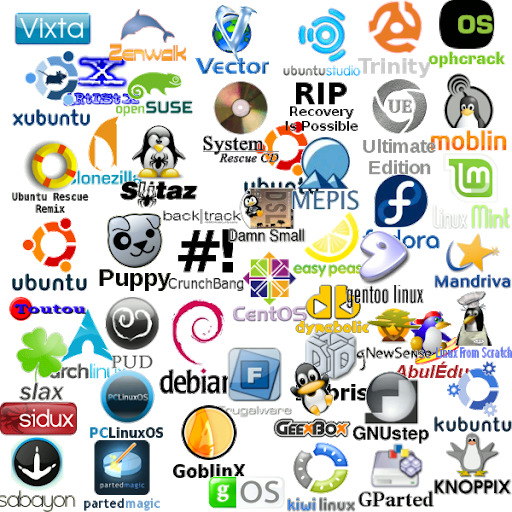
\includegraphics[width=.9\textwidth]{linux_distros}

      \tiny{Source: wikimedia.org}

    \end{column}
    \begin{column}{.55\textwidth}
      Open source: code accessible à tous \bigskip 

      Forces de l'open source:
      \begin{itemize}
        \item Performances
        \item
              Personnalisation
        \item Support communautaire
        \item Sécurité
        \item Transparence
        \item Gratuité
      \end{itemize}

      \bigskip 

      Attention: choix de la distribution, compatibilité 

    \end{column}
  \end{columns}
\end{frame}

\begin{frame}{Raspberry Pi OS}{Distribution Linux officielle}
  
\includegraphics[width=.7\textwidth]{raspberry_os} 

  \bigskip
  \begin{itemize}
    \item Basée sur Debian (très stable)
    \item Optimisée
          pour Raspberry Pi
    \item Utilisé par une large communauté
  \end{itemize}
\end{frame}

\begin{frame}{Parés au démarrage!
  }{Attachez vos câbles}

  \begin{enumerate}
    \item Vérifier la carte SD
    \item Brancher:
          \begin{itemize}
            \item Ecran
            \item Clavier
            \item Souris
            \item Alimentation
          \end{itemize}
    \item Bienvenue dans Raspberry Pi OS!
  \end{enumerate}
\end{frame}

\begin{frame}{Le bureau Raspberry Pi OS}{Familier?
    Tant mieux!
  }
  \centering 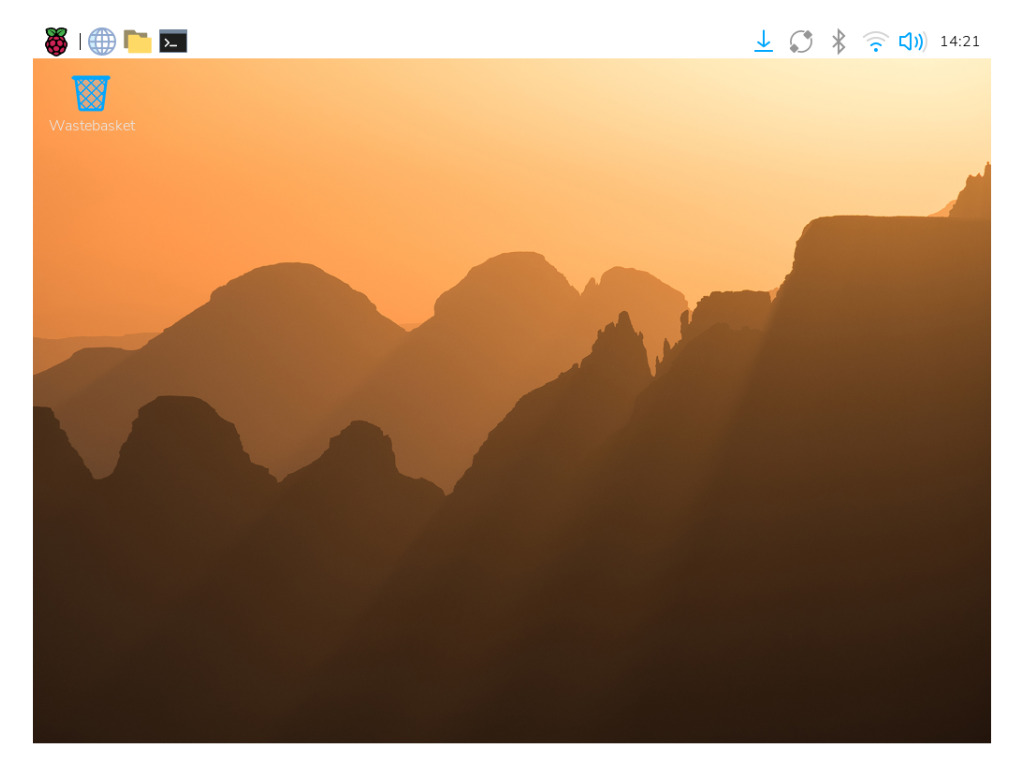
\includegraphics[width=.6\textwidth]{home}
\end{frame}
\begin{frame}{Le bureau Raspberry Pi OS}{Menu démarrer}
  \centering 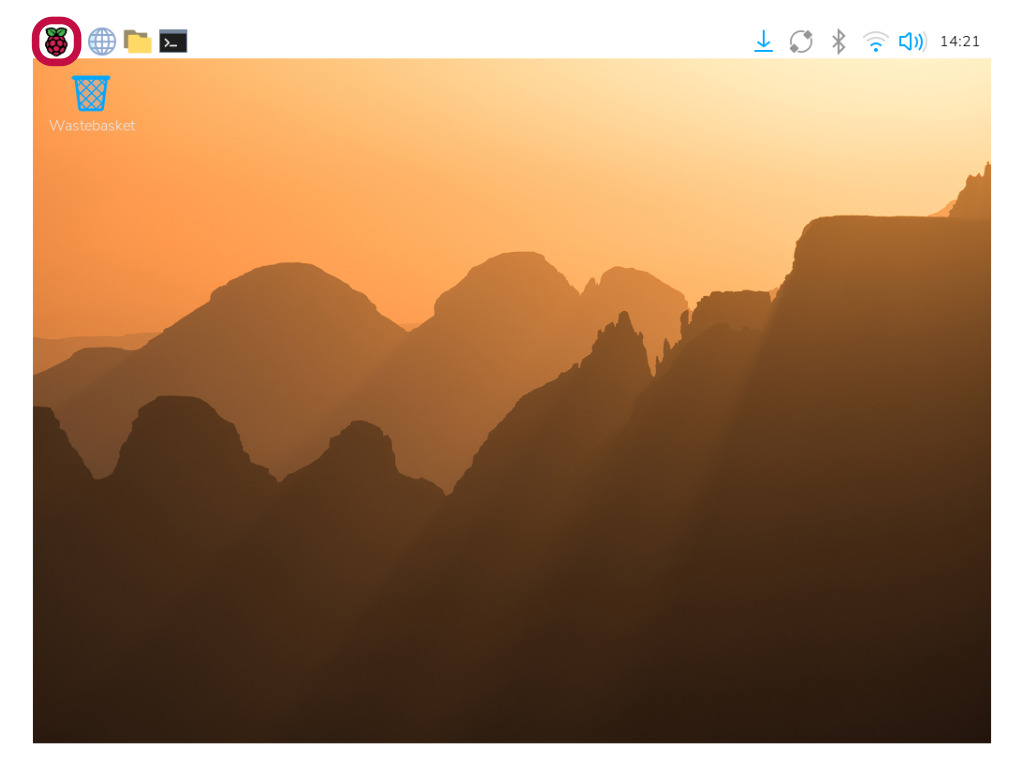
\includegraphics[width=.6\textwidth]{home_start}
\end{frame}
\begin{frame}{Le bureau Raspberry Pi OS}{Navigateur internet}
  \centering 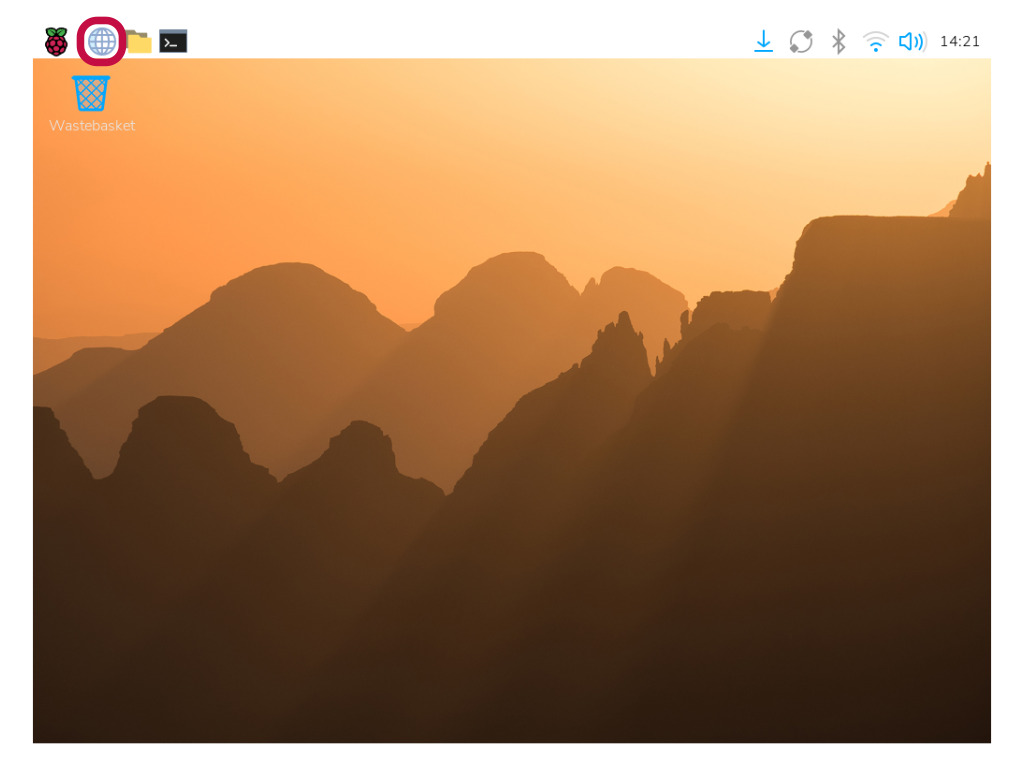
\includegraphics[width=.6\textwidth]{home_web}
\end{frame}
\begin{frame}{Le bureau Raspberry Pi OS}{Explorateur de fichiers}
  \centering 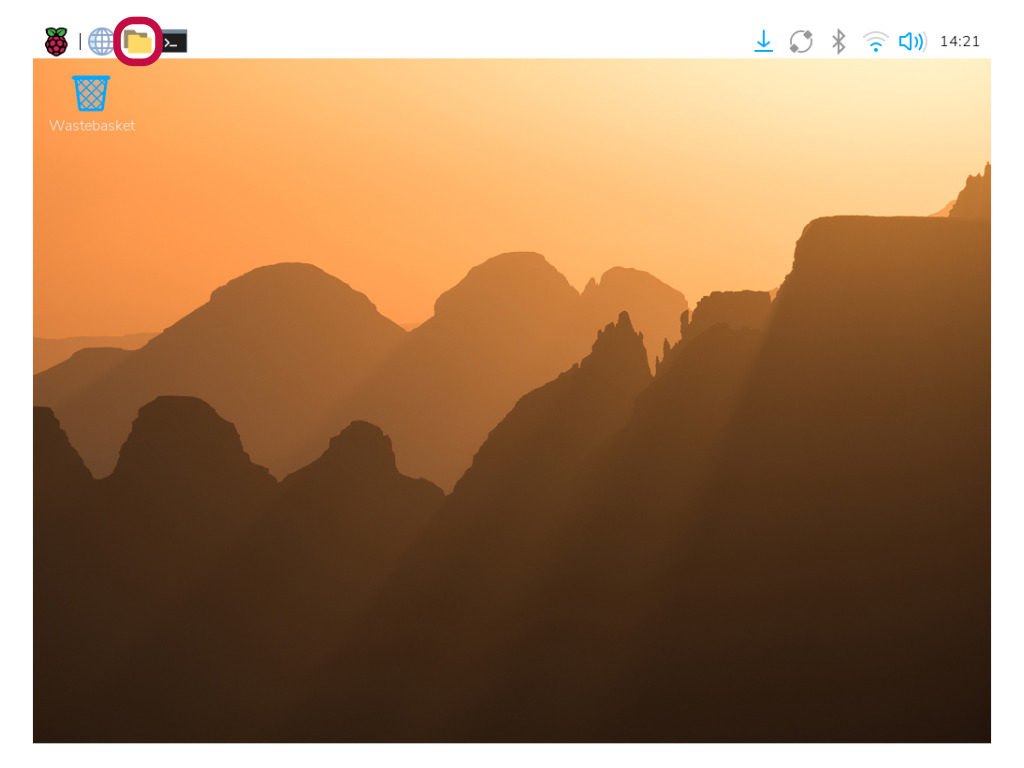
\includegraphics[width=.6\textwidth]{home_files}
\end{frame}
\begin{frame}{Le bureau Raspberry Pi OS}{Terminal, c'est pour plus tard!}
  \centering 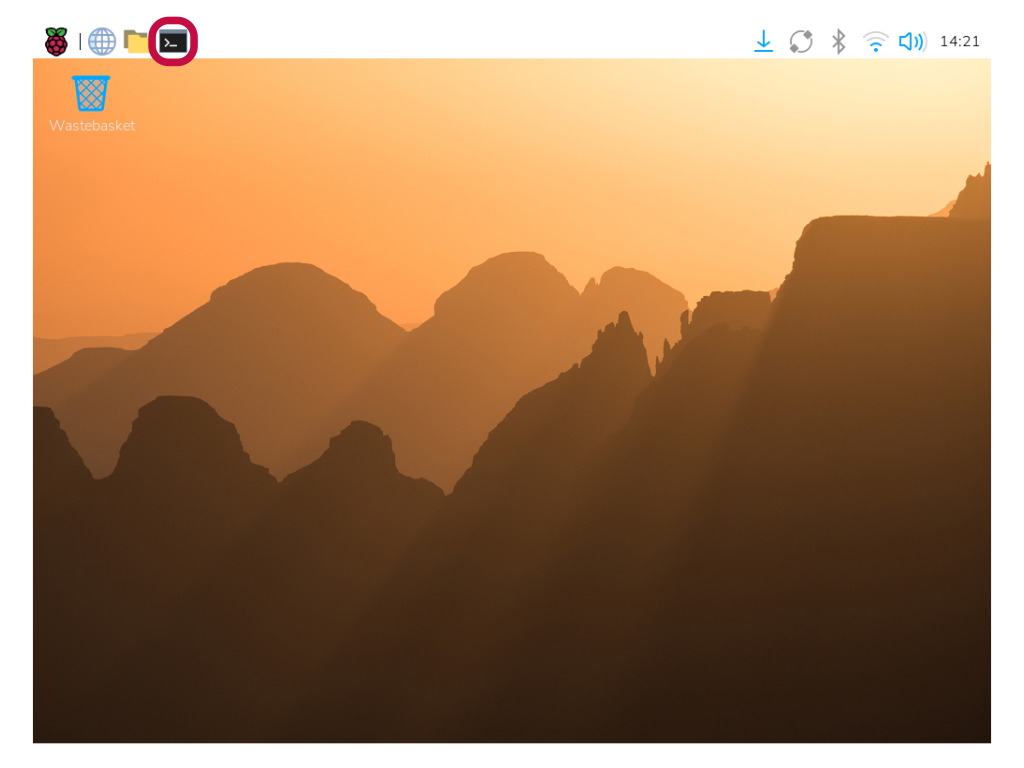
\includegraphics[width=.6\textwidth]{home_term}
\end{frame}
\begin{frame}{Le bureau Raspberry Pi OS}{Mises à jour}
  \centering 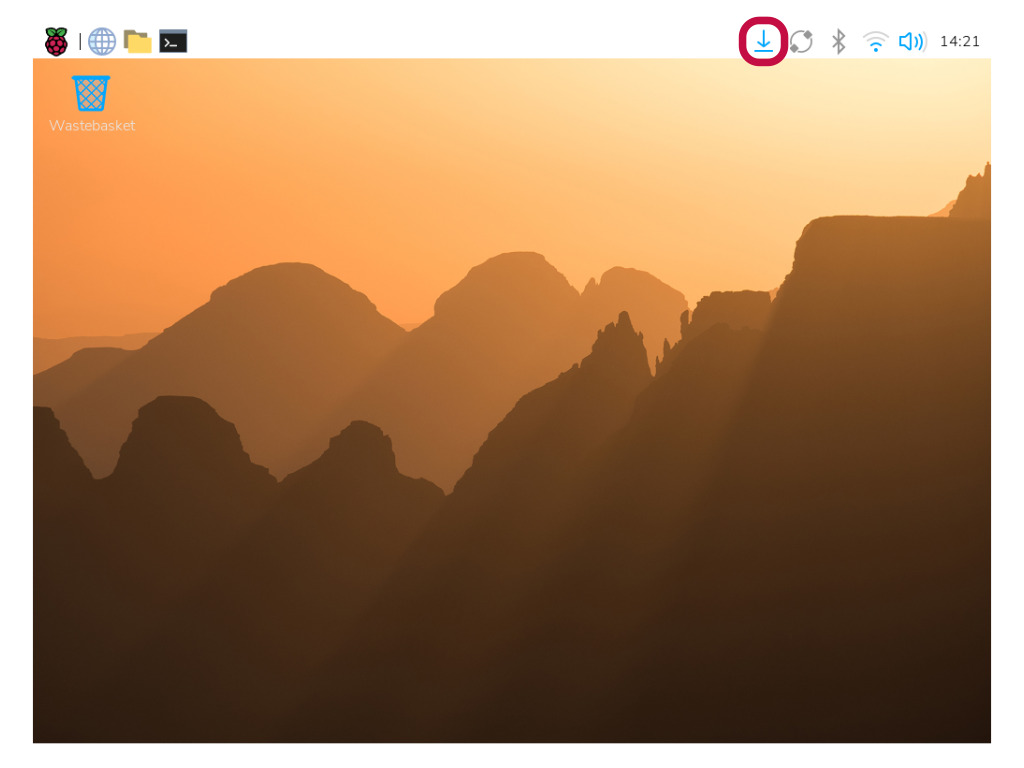
\includegraphics[width=.6\textwidth]{home_updates}
\end{frame}
\begin{frame}{Le bureau Raspberry Pi OS}{Wi-Fi}
  \centering 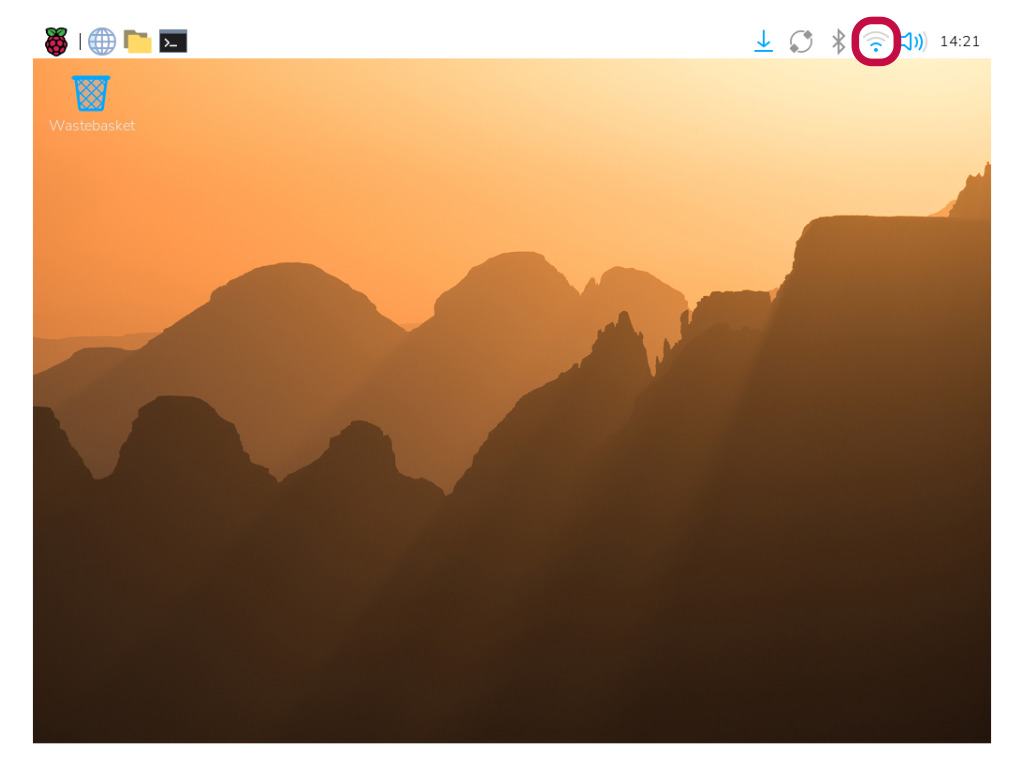
\includegraphics[width=.6\textwidth]{home_wifi}
\end{frame}
\begin{frame}{Le bureau Raspberry Pi OS}{Corbeille}
  \centering 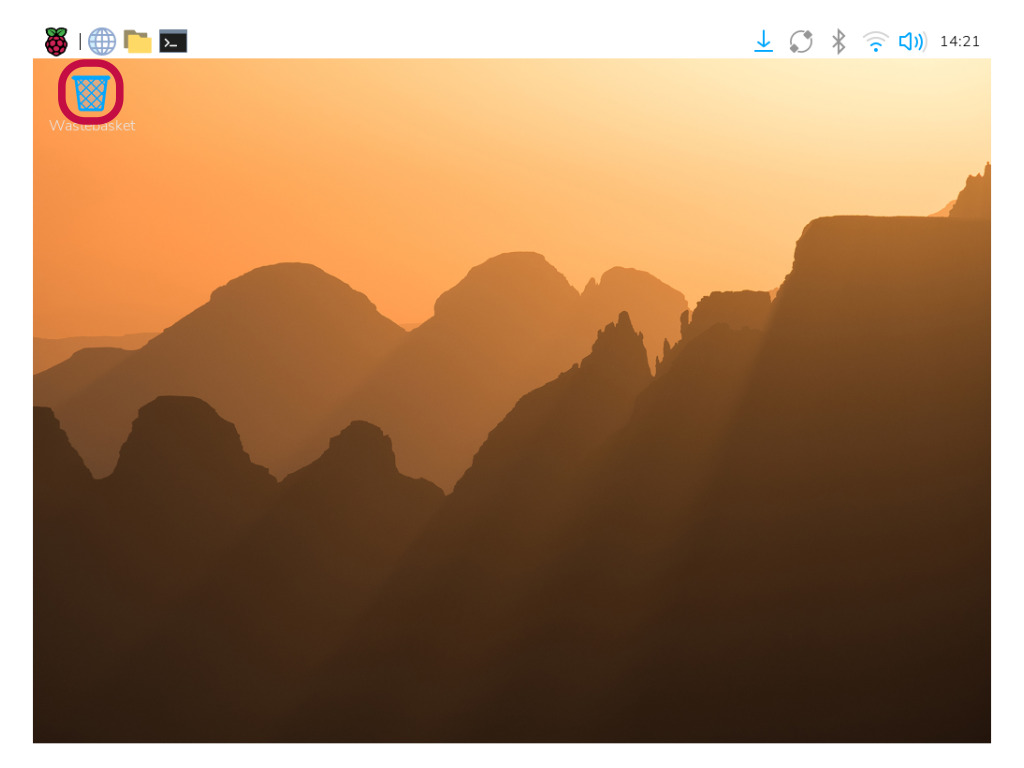
\includegraphics[width=.6\textwidth]{home_trash}
\end{frame}

\begin{frame}{Exercice du jour}{À vos claviers!}
  \begin{enumerate}
    \item  Changer la langue du système en français
          \begin{itemize}
            \item Menu démarrer \(\rightarrow\) Paramètres \(\rightarrow\)
                  Localisation
          \end{itemize}
    \item Redémarrer le Raspberry Pi (proprement, pas en débranchant!)
    \item Configurer la résolution d'écran
          \begin{itemize}
            \item Menu démarrer \(\rightarrow\) Paramètres \(\rightarrow\)
                  Écran
          \end{itemize}
    \item Vérifier que le Wi-Fi est connecté (SSID: electroLAB, mot de passe:
          7N5GGI79)
    \item Vérifier qu'internet marche via le navigateur
    \item Mettre à jour le système
    \item Trouver combien de mémoire RAM est utilisée
    \item Créer un fichier texte avec Geany
    \item Changer le nom d'hôte (hostname) du Raspberry Pi
          \begin{itemize}
            \item Menu démarrer \(\rightarrow\) Paramètres \(\rightarrow\)
                  Système
            \item Est-ce que ça a marché?
                  Même après redémarrage?
          \end{itemize}

  \end{enumerate}

\end{frame}

\begin{frame}{\strut}
  \centering \alert{\huge Vos idées de projets?}
\end{frame}

\begin{frame}{Des idées à explorer avec Raspberry Pi}
  \begin{itemize}
    \item Objets connectés (IoT), avec capteurs et logique embarquée
    \item Simulateur de console de jeux rétro
    \item Serveur domotique entièrement personnalisable
    \item VPN personnel pour naviguer en sécurité
    \item Appareil multimédia dédié (pour la musique, les films, etc.)
    \item Un bloqueur de publicités sur votre réseau
    \item Un ordinateur ultraportable pour le télétravail
    \item Un hotspot Wi-Fi sécurisé transportable
    \item Une plateforme pour l'art numérique (photographie, son, interactions)
  \end{itemize}

\end{frame}

\end{document}
